\documentclass{article}
\usepackage[utf8]{inputenc}
\usepackage{amsmath,amsfonts,amssymb} % Paquetes para matemáticas
\usepackage{ulem} % Para subrayar texto
\usepackage{geometry}
\usepackage{indentfirst}
\usepackage{graphicx}
\usepackage{float}

\geometry{
    a4paper,
    left=2cm,
    right=2cm,
    top=2.5cm,
    bottom=2.5cm,
    includefoot,
    headheight=15pt,
    headsep=0.5cm,
    footskip=1cm
}

\title{Métodos Computacionales - TP1}
\author{Josefina Jahde, Dafydd Jenkins}
\date{\today}

\begin{document}

\maketitle

\section*{Introducción}
El siguiente informe detalla las tareas realizadas para la resolución del trabajo práctico: cómo fueron resueltas las consignas, los desarrollos de las mismas, los resultados de los experimentos y conclusiones.


\section*{Ejercicio 1}
Las función solicitada en el primer ítem se encuentra en el archivo .ipynb adjunto, definida como f0(t, puntos).
Para el segundo ítem, se partió de la formula:

$$
g(t) = (1 - t)f_0(t) + t f_1(t)
$$

La desarrollamos como se muestra en la imágen:

\begin{figure}[H]
    \centering
    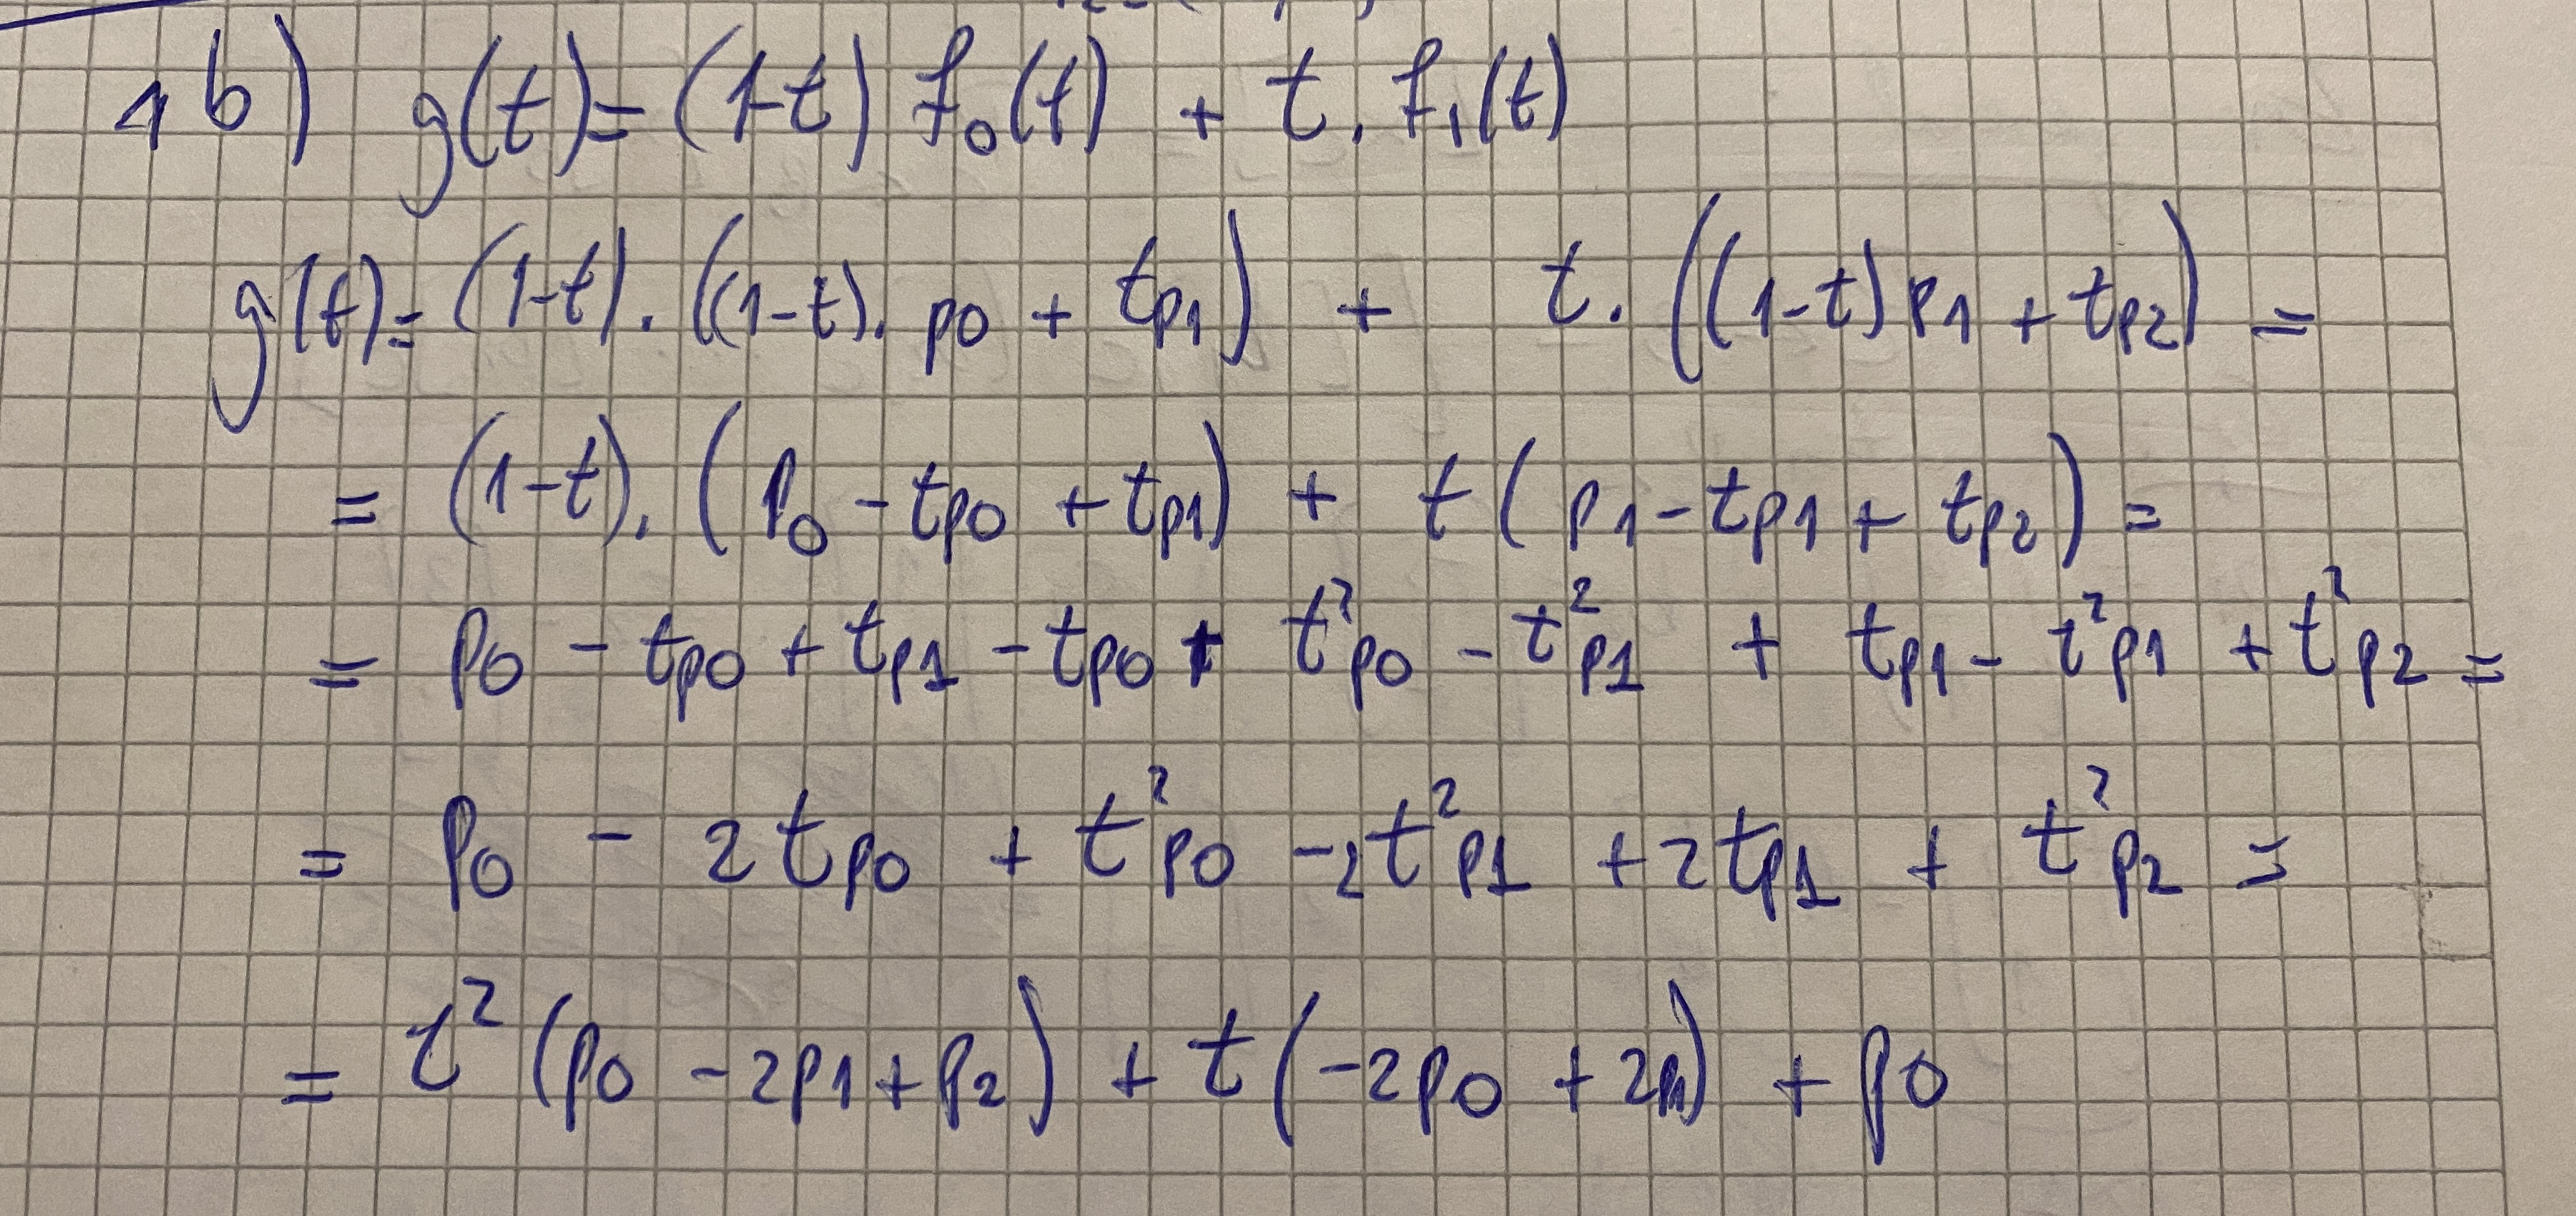
\includegraphics[width=0.6\textwidth]{imagenes/1b.jpg}
    \caption{Desarrollo de $g(t)$}
    \label{fig:ejemplo}
\end{figure}

Llegando a la fórmula final:

$$
g(t) = t^2 (p_0 - 2 p_1 + p_2) + t (-2 p_0 + 2 p_1) + p_0
$$

Como se puede ver, la fórmula obtenida es cuadrática con respecto a $t$, por lo tanto, $g(t)$ es una curva de Bézier cuadrática.
Para el tercer inciso,el gráfico se generó con el código que se encuentra en la sección "Ejercicio 1". Como puntos de ejemplo se usaron $p_0 = (1, 2)$, $p_1 = (5, 6)$, $p_2 = (2, 10)$. El gráfico resultante se muestra  a continuación:

\begin{figure}[H]
    \centering
    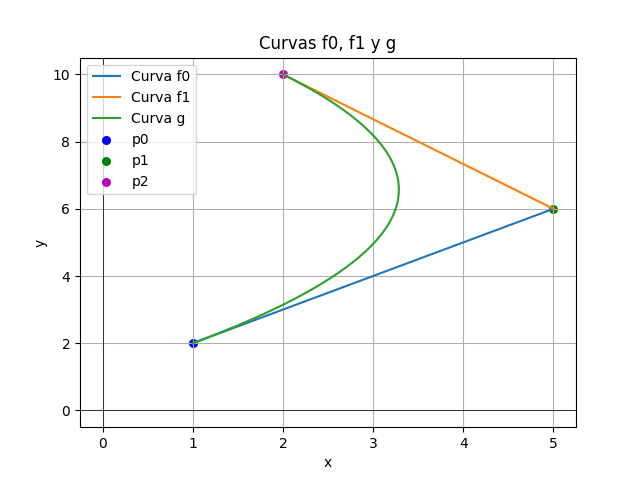
\includegraphics[width=0.6\textwidth]{imagenes/graf_ej1.png}
    \caption{$f_0(t)$, $f_1(t)$ y $g(t)$ con puntos de ejemplo}
    \label{fig:ejemplo}
\end{figure}

Luego de construir $g(t)$ a partir de $f_0(t)$ y $f_1(t)$ podemos decir que estas dos últimaas "se combinan" para generar  $g(t)$. A los resultados de $f_0(t)$ y $f_1(t)$ se les vuelve a aplicar la misma función (porque $f_0(t)$ y $f_1(t)$ son la misma función aplicada sobre distintos puntos).

Decidimos definir "la función" como $f(t, p_i, p_j) = (1-t) p_i + t p_j$.

Entonces, $f_0(t) = f(t, p_0, p_1)$, $f_1(t) = f(t, p_1, p_2)$ y $g(t) = f(t, f_0(t), f_1(t))$.

Intuímos que para generar una curva de Bézier cúbica, se agregará un cuarto punto $p_3$. el mismo se combinará con $p_2$ para formar una $f_2(t) = f(t, p_2, p_3)$. El resultado de esa función se combinara con el de $f_1(t)$ para formar una función similar a $g(t)$. El resultado de estas dos "$g(t)$" serán utilizados como parámetros nuevamente de $f(t, p_i, p_j)$ para generar la curva de Bézier cúbica.

\section*{Ejercicio 2}

Para el primer ítem, partimos de la definición de $h(t) = (1 - t)g_1(t) + t g_2(t)$. La desarrollamos como se muestra a continuación:

\begin{figure}[H]
    \centering
    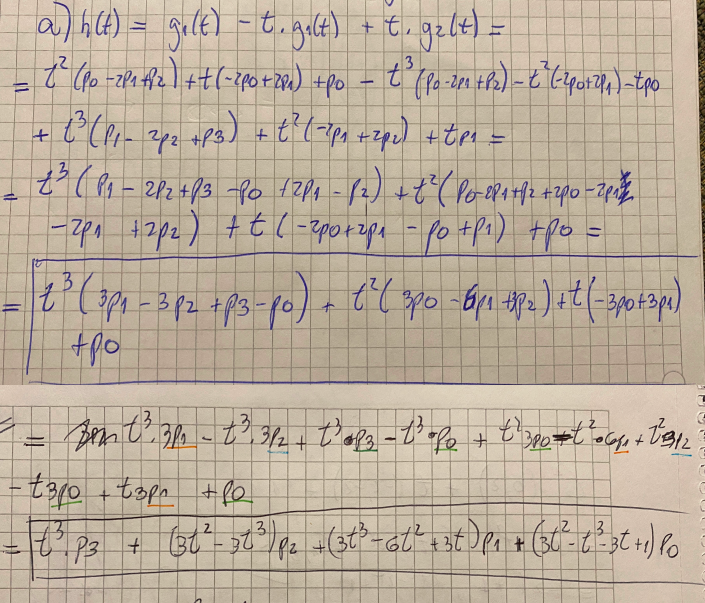
\includegraphics[width=0.6\textwidth]{imagenes/2a.png}
    \caption{Desarrollo de $h(t)$}
    \label{fig:ejemplo}
\end{figure}

Llegando a la fórmula final:

$$
h(t) = t^3p_3 + (3t^2-3t^3)p_2 + (3t^3-6t^2+3t)p1 + (3t^2-t^3-3t+1)p0
$$

Para el segundo ítem, utilizamos el código que se puede encontrar en la sección "Ejercicio 2" del archivo .ipynb. El gráfico resultante es el siguiente:

\begin{figure}[H]
    \centering
    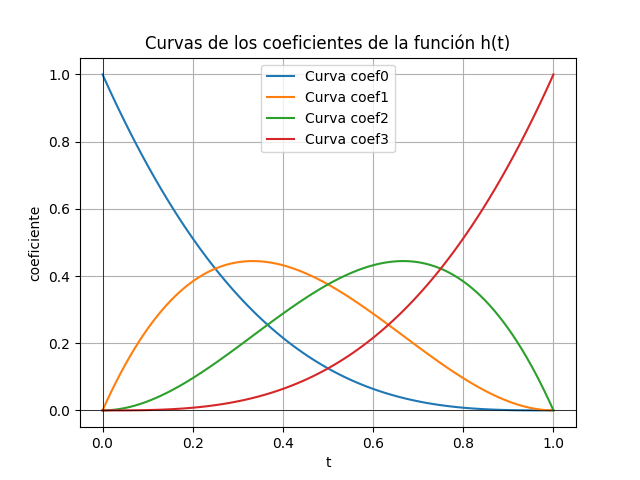
\includegraphics[width=0.6\textwidth]{imagenes/graf_2a.png}
    \caption{Coeficientes de $h(t)$}
    \label{fig:ejemplo}
\end{figure}

Para la suma de los coeficientes, vimos que con $t=0.3, t=0.5 y t=0.8$ dicha suma siempre daba 1. Por lo tanto decidimos ver que pasaba con un t genérico. La suma de los coeficientes será:

$$
t^3 + 3t^2-3t^3 + 3t^3-6t^2+3t +3t^2-t^3-3t+1
$$

En dicha suma, los términos dependientes de t se cancelan para toda t, por lo que la suma siempre vale 1.

Para el tercer ítem, se obtuvo, a partir del código en el archivo .ipynb en la sección "Ejercicio 2", el siguiente gráfico:

\begin{figure}[H]
    \centering
    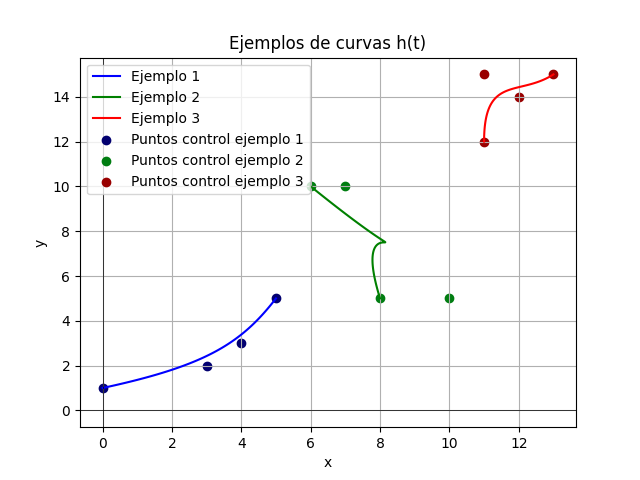
\includegraphics[width=0.6\textwidth]{imagenes/graf_2c.png}
    \caption{Ejemplos de $h(t)$ con puntos de control aleatorios}
    \label{fig:ejemplo}
\end{figure}

\section*{Ejercicio 3:}

\subsection*{Primer ítem:}
Para $S_1 = {v_1}$, las posibles combinaciones lineales son $c_1 v_1$. Como la suma de los coeficientes debe ser 1, y solo hay un coeficiente, debe valer $c_1 = 1$. Por lo tanto, $conv(S_1) = {v_1}$. Visualización para $v_1 =$ (1, 2)
 
Para $S_2 = {v_1, v_2}$, las posibles combinaciones lineales son $c_1 v_1 + c_2 v_2$. Como la suma de los coeficientes debe ser 1, debe valer $c_1 + c_2= 1 \iff c_1 = 1 - c_2$. Por lo tanto, $conv(S_2) = \{c_1 v_1+ c_2 v_2 \in \mathbb{R}^2 / c_1, c_2 > 0$ y $ c_1 = 1- c_2\} = \{$[$v_1, v_2$][$1-c_2, c_2$]$^T$\}.

Para $S_3 = {v_1, v_2, v_3}$, las posibles combinaciones lineales son $c_1 v_1 + c_2 v_2 + c_3 v_3$. Como la suma de los coeficientes debe ser 1, debe valer $c_1 + c_2 + c_3 = 1 \iff c_1 = 1 - c_2 - c_3$ (hay dos variables libres). Por lo tanto, $conv(S_3) = \{c_1 v_1+ c_2 v_2 + c_3 v_3\in \mathbb{R}^2 / c_1, c_2, c_3 > 0$ y $ c_1 = 1- c_2-c_3\} = \{$[$v_1, v_2, v_3$][$1-c_2 - c_3, c_2, c_3$]$^T$\}.

Visualizaciiones:

\begin{figure}[H]
   \centering
    \begin{minipage}{0.45\textwidth}
        \centering
        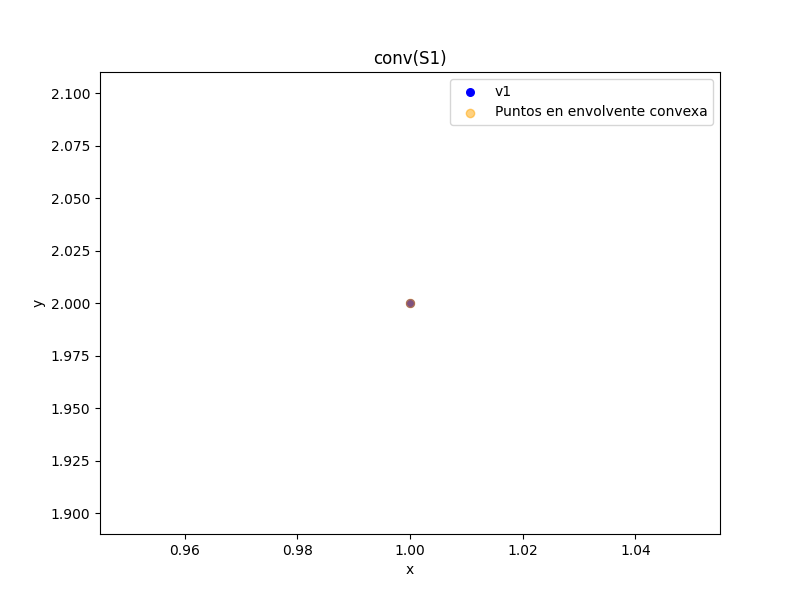
\includegraphics[width=\textwidth]{imagenes/conv(s1).png}
        \caption{conv(s1)}
        \label{fig:grafico1}
    \end{minipage}
    \hfill
    \begin{minipage}{0.45\textwidth}
        \centering
        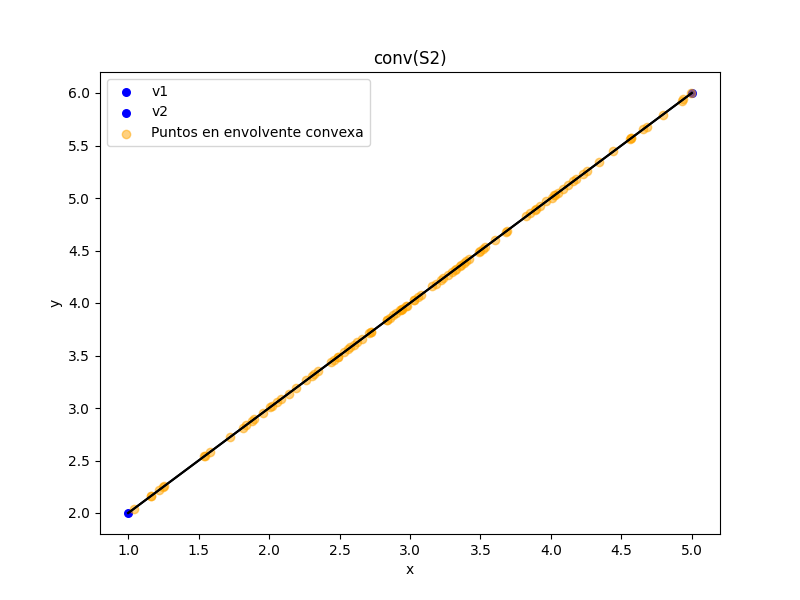
\includegraphics[width=\textwidth]{imagenes/conv(s2).png}
        \caption{conv(s2)}
        \label{fig:grafico2}
    \end{minipage}
\begin{minipage}{0.45\textwidth}
        \centering
        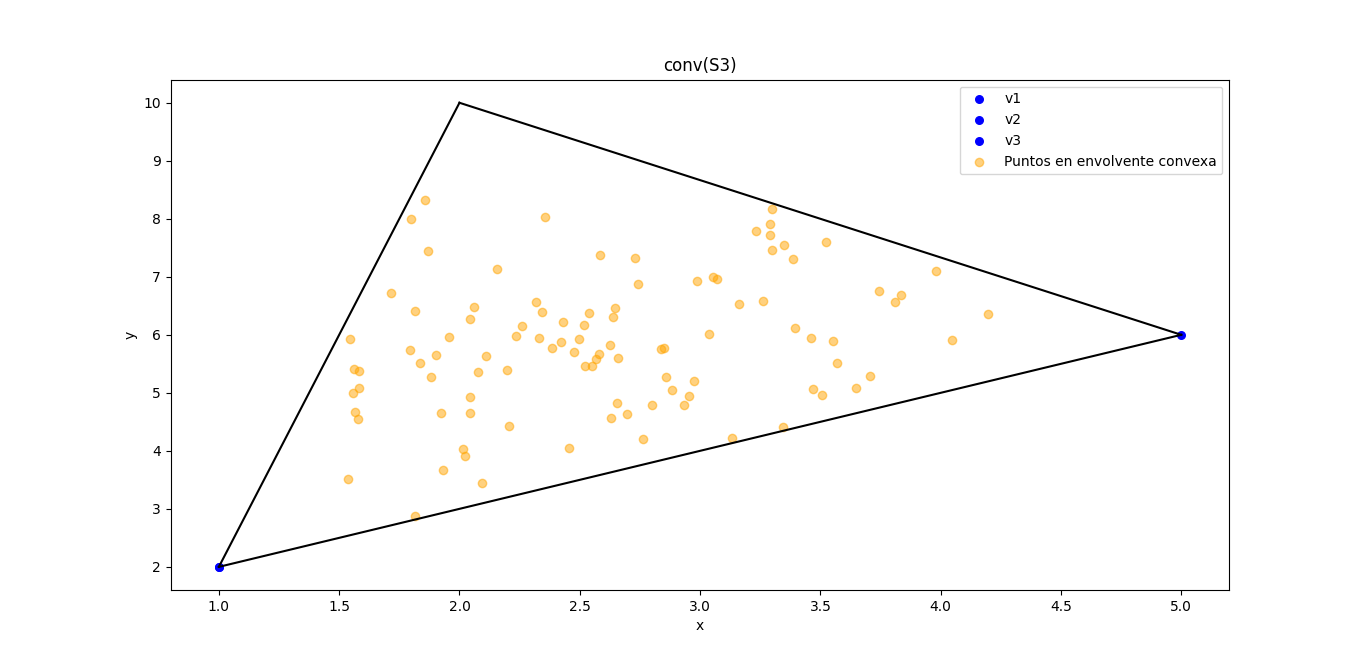
\includegraphics[width=\textwidth]{imagenes/conv(s3).png}
        \caption{conv(s3)}
        \label{fig:grafico3}
    \end{minipage}
    \label{fig:tres_graficos}
\end{figure}

Como se puede ver, las combinaciones convexas siempre están contenidas en el polígono que forman los puntos combinados (marcado en cada caso, salvo el de $S_1$ en negro).

\subsection*{Segundo ítem:}
Las curvas de Bézier son combinaciones convexas ya que, como demostramos en el ejercicio 2, la suma de los coeficientes que mutiplican a los puntos siempre suman 1 y son $>=0$ para todo t entre 0 y 1. Por lo tanto, como en el ítem anterior, los puntos que resulten de ellas siempre estarán dentro del polígono delimitado por los puntos combinados, es decir, los puntos de control. Se muestran algunos ejeplos (generados corriendo varias veces el código del archivo .ipynb en la sección "Ejercicio 3"):

\begin{figure}[H]
   \centering
    \begin{minipage}{0.45\textwidth}
        \centering
        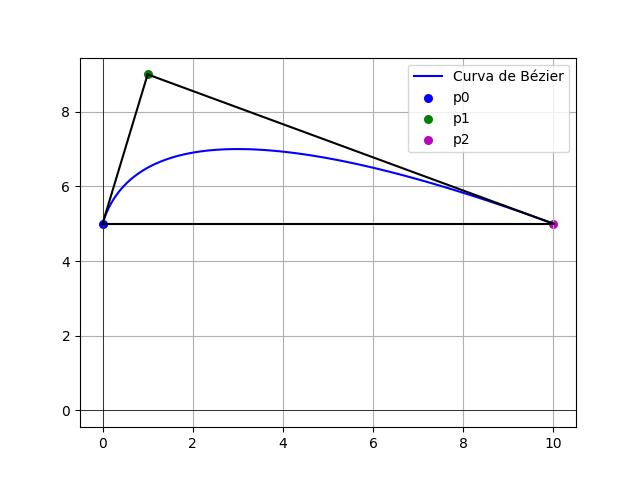
\includegraphics[width=\textwidth]{imagenes/3b1.png}
        \caption{Ejemplo 1 Bézier con 3 puntos}
        \label{fig:grafico1}
    \end{minipage}
    \hfill
    \begin{minipage}{0.45\textwidth}
        \centering
        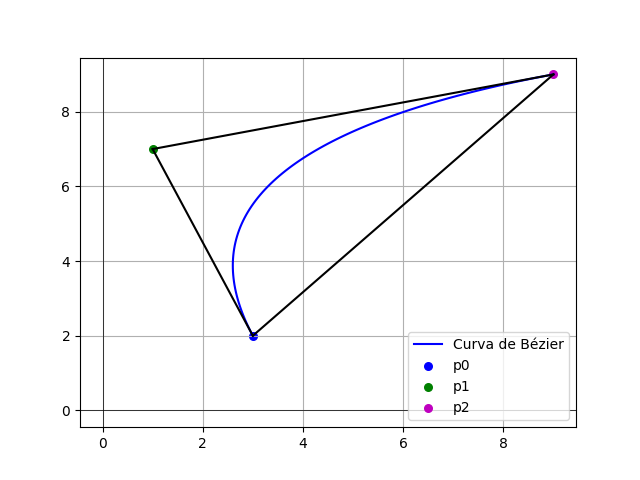
\includegraphics[width=\textwidth]{imagenes/3b2.png}
        \caption{Ejemplo 2 Bézier con 3}
        \label{fig:grafico2}
    \end{minipage}
\begin{minipage}{0.45\textwidth}
        \centering
        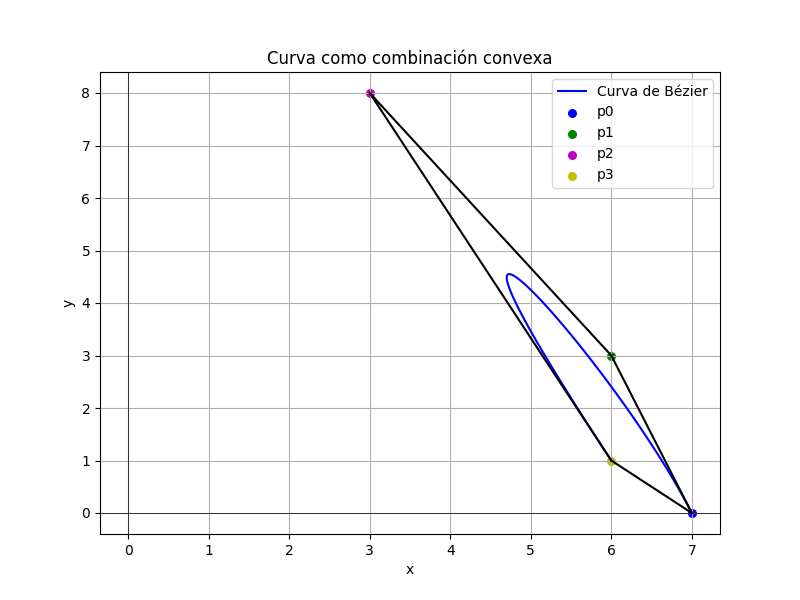
\includegraphics[width=\textwidth]{imagenes/3b3.png}
        \caption{Ejemplo 1 Bézier con 4 puntos}
        \label{fig:grafico3}
    \end{minipage}
\begin{minipage}{0.45\textwidth}
        \centering
        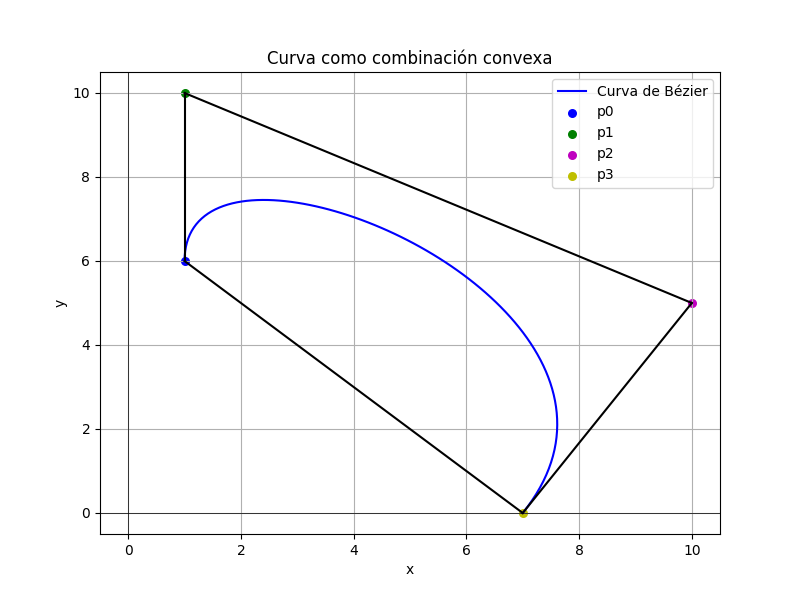
\includegraphics[width=\textwidth]{imagenes/3b4.png}
        \caption{Ejemplo 2 Bézier con 4 puntos}
        \label{fig:grafico3}
    \end{minipage}
    \label{fig:tres_graficos}
\end{figure}

\textbf{Observación:} Si al correr el código para generar los gráficos el polígono de la curva con 4 puntos de control se cruza con la curva, notar que se puede dibujar otro polígono delimitado por los puntos de control que si contiene a la curva en su totalidad.

\section*{Ejercicio 4:}
Para escribri la forma paramétrica de $x(t)$ como  $x(t) = G M_B u(t)$ donde $u(t) =
\left[ 
\begin{array}{c}
1 \\
t \\
t^2 \\
t^3
\end{array}
\right]
$, primero la desarrollamos obteniendo:

$$
x(t) = p_0 + t(-3p_0+3p_1) + t^2(3p_0-6p_1+3p_2) + t^3(-p_0+3p_1-3p_2+p_3)
$$

Con esta forma se puede ver más claramente como descomponer a  $x(t)$ como  $x(t) = G M_B u(t)$. La descomposición obtenida fue:

$$
x(t) = 
\begin{bmatrix}
p_0 & p_1 & p_2 & p_3
\end{bmatrix}
\begin{bmatrix}
1 & -3 & 3 & -1 \\
0 & 3 & -6 & 3 \\
0 & 0 & 3 & -3 \\
0 & 0 & 0 & 1
\end{bmatrix}
\begin{bmatrix}
1 \\
t \\
t^2 \\
t^3
\end{bmatrix}
$$

Para calcular $x'(t)$ y $x''(t)$  derivamos el vector $u(t)$ con respecto a t. De esta forma obtuvimos $u'(t) =
\begin{bmatrix}
0 \\ 1 \\ 2t \\ 3t^2
\end{bmatrix}
$ y $u''(t) =
\begin{bmatrix}
0 \\ 0 \\ 2 \\ 6t
\end{bmatrix}
$

Con esto, $x'(t) = G M_B u'(t)$ y $x'(t) = G M_B u''(t)$. Se desarrollaron estas expresiones como se muestra a continuación para llegar a una expresión desarrollada de $x'(t)$ y $x''(t)$.

\begin{figure}[H]
   \centering
    \begin{minipage}{0.45\textwidth}
        \centering
        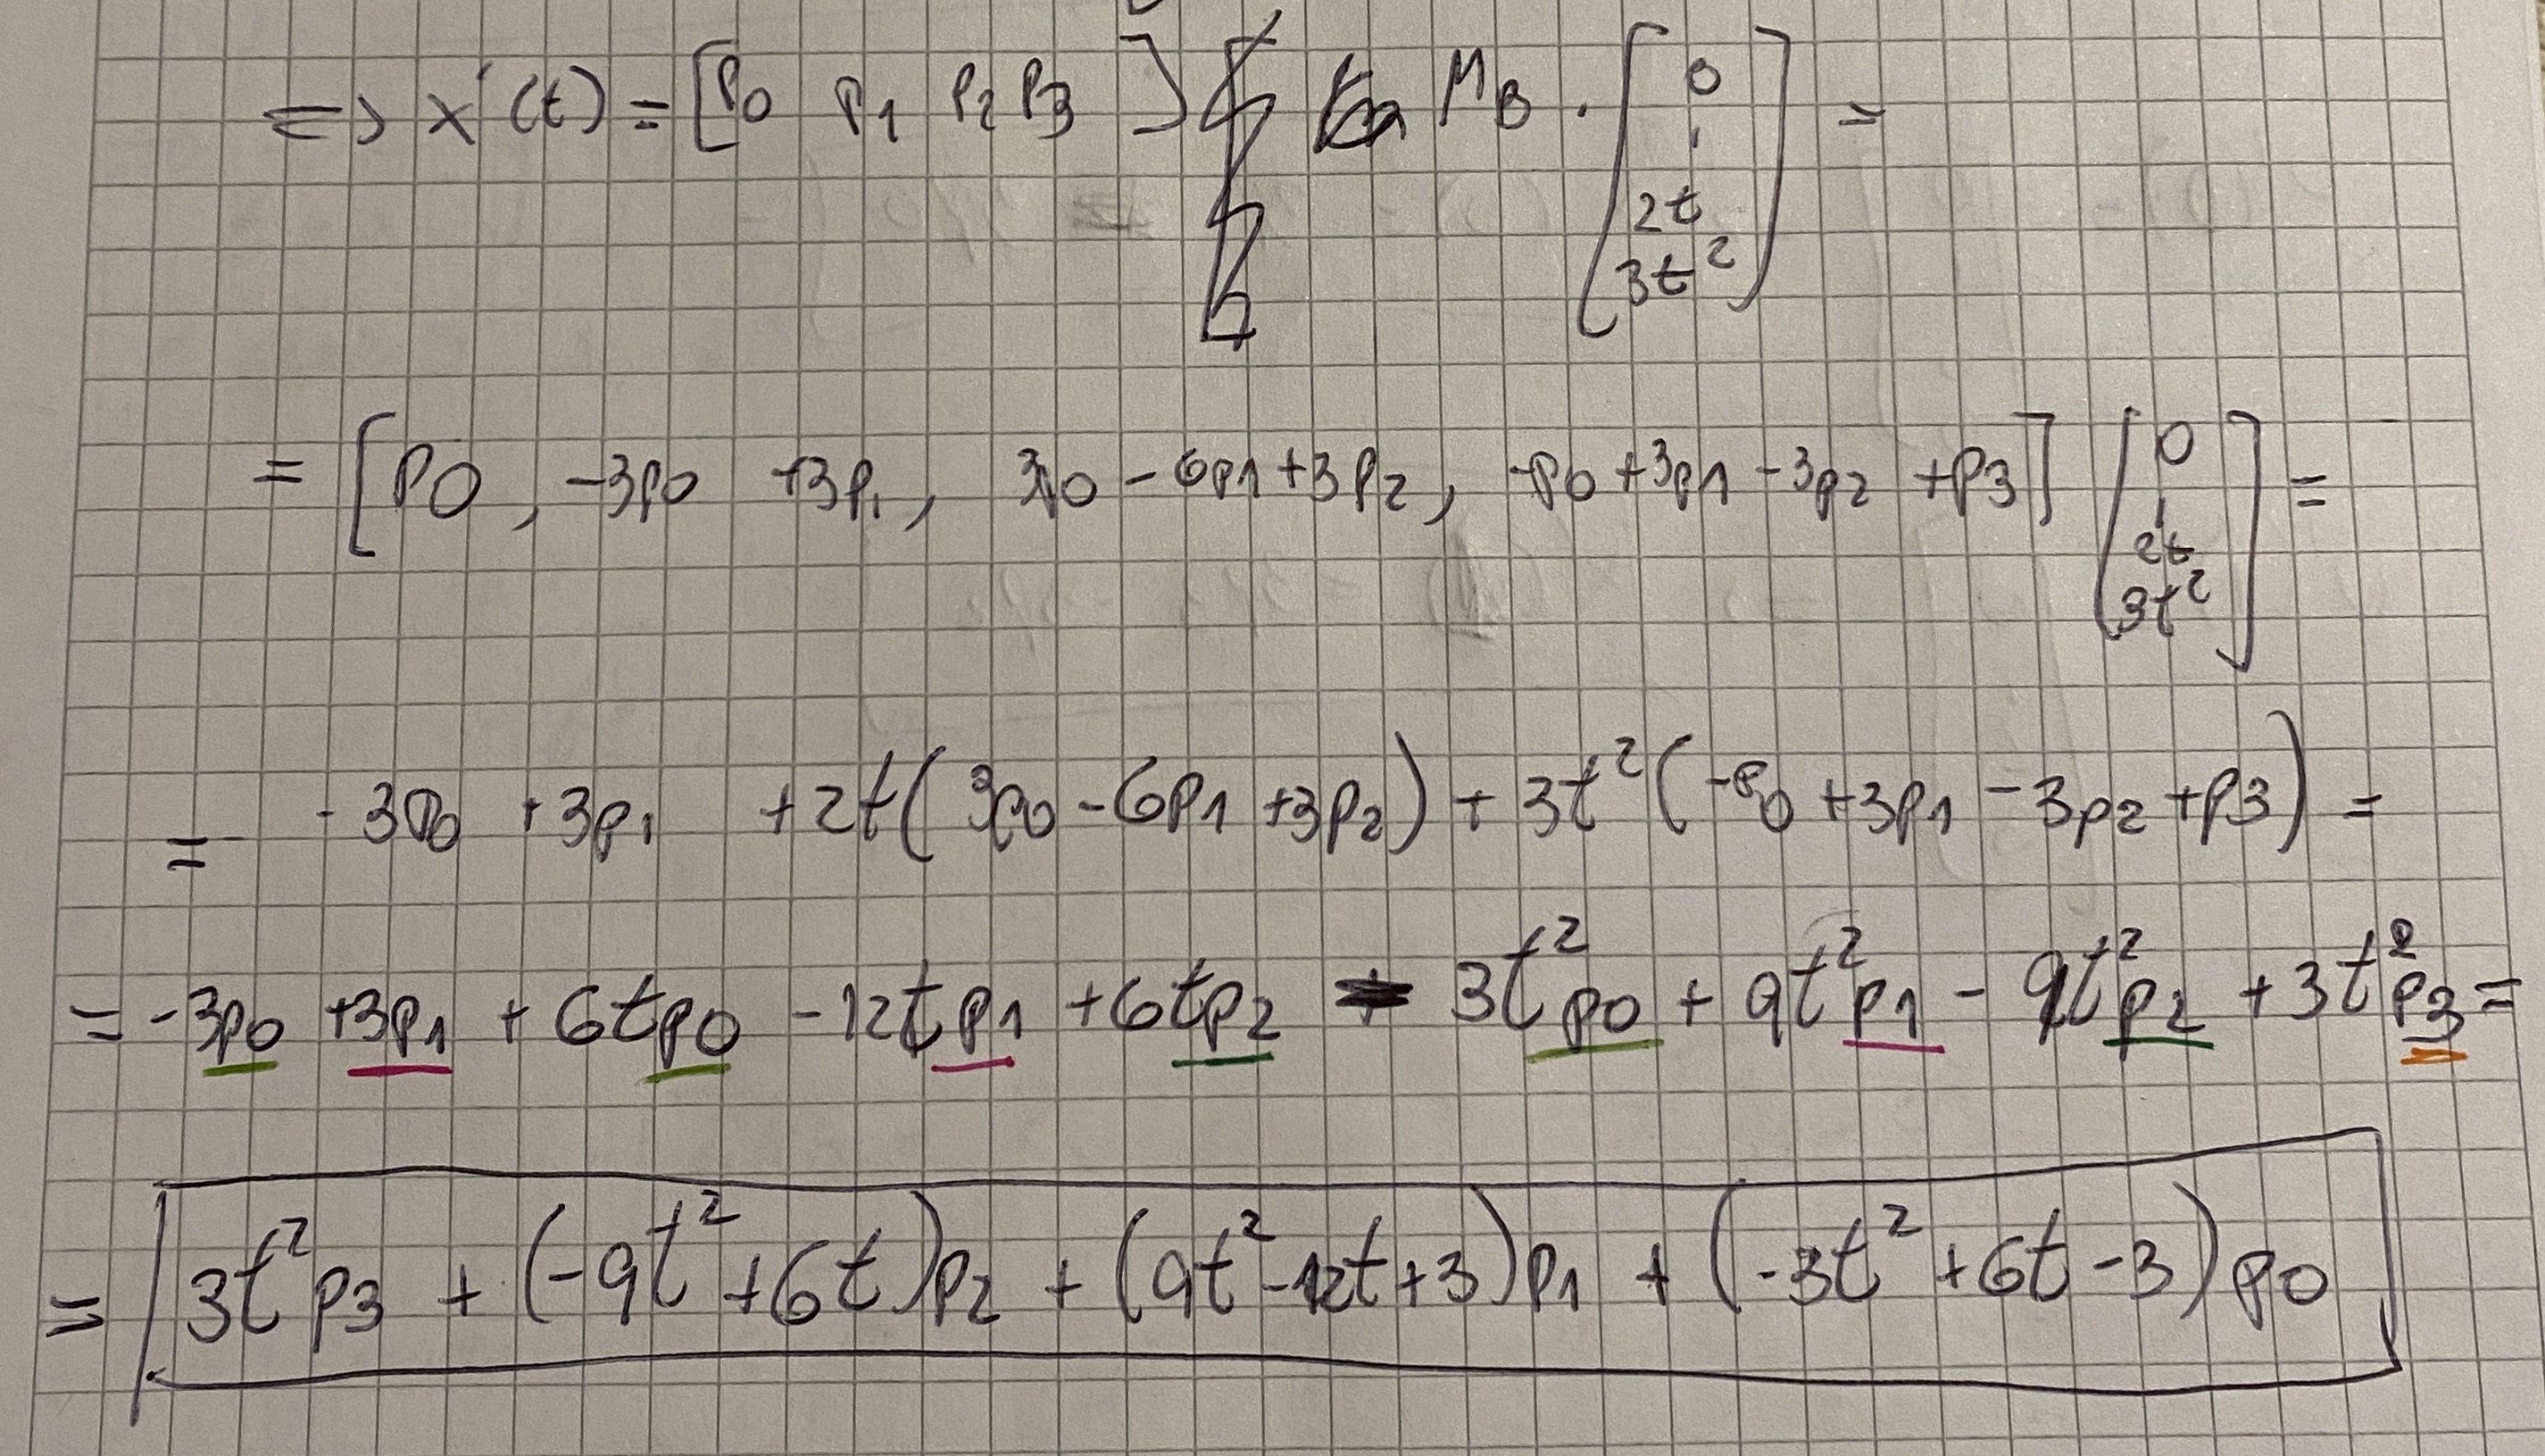
\includegraphics[width=\textwidth]{imagenes/primderiv.jpg}
        \caption{Desarrollo de $x'(t)$}
        \label{fig:grafico1}
    \end{minipage}
    \hfill
    \begin{minipage}{0.45\textwidth}
        \centering
        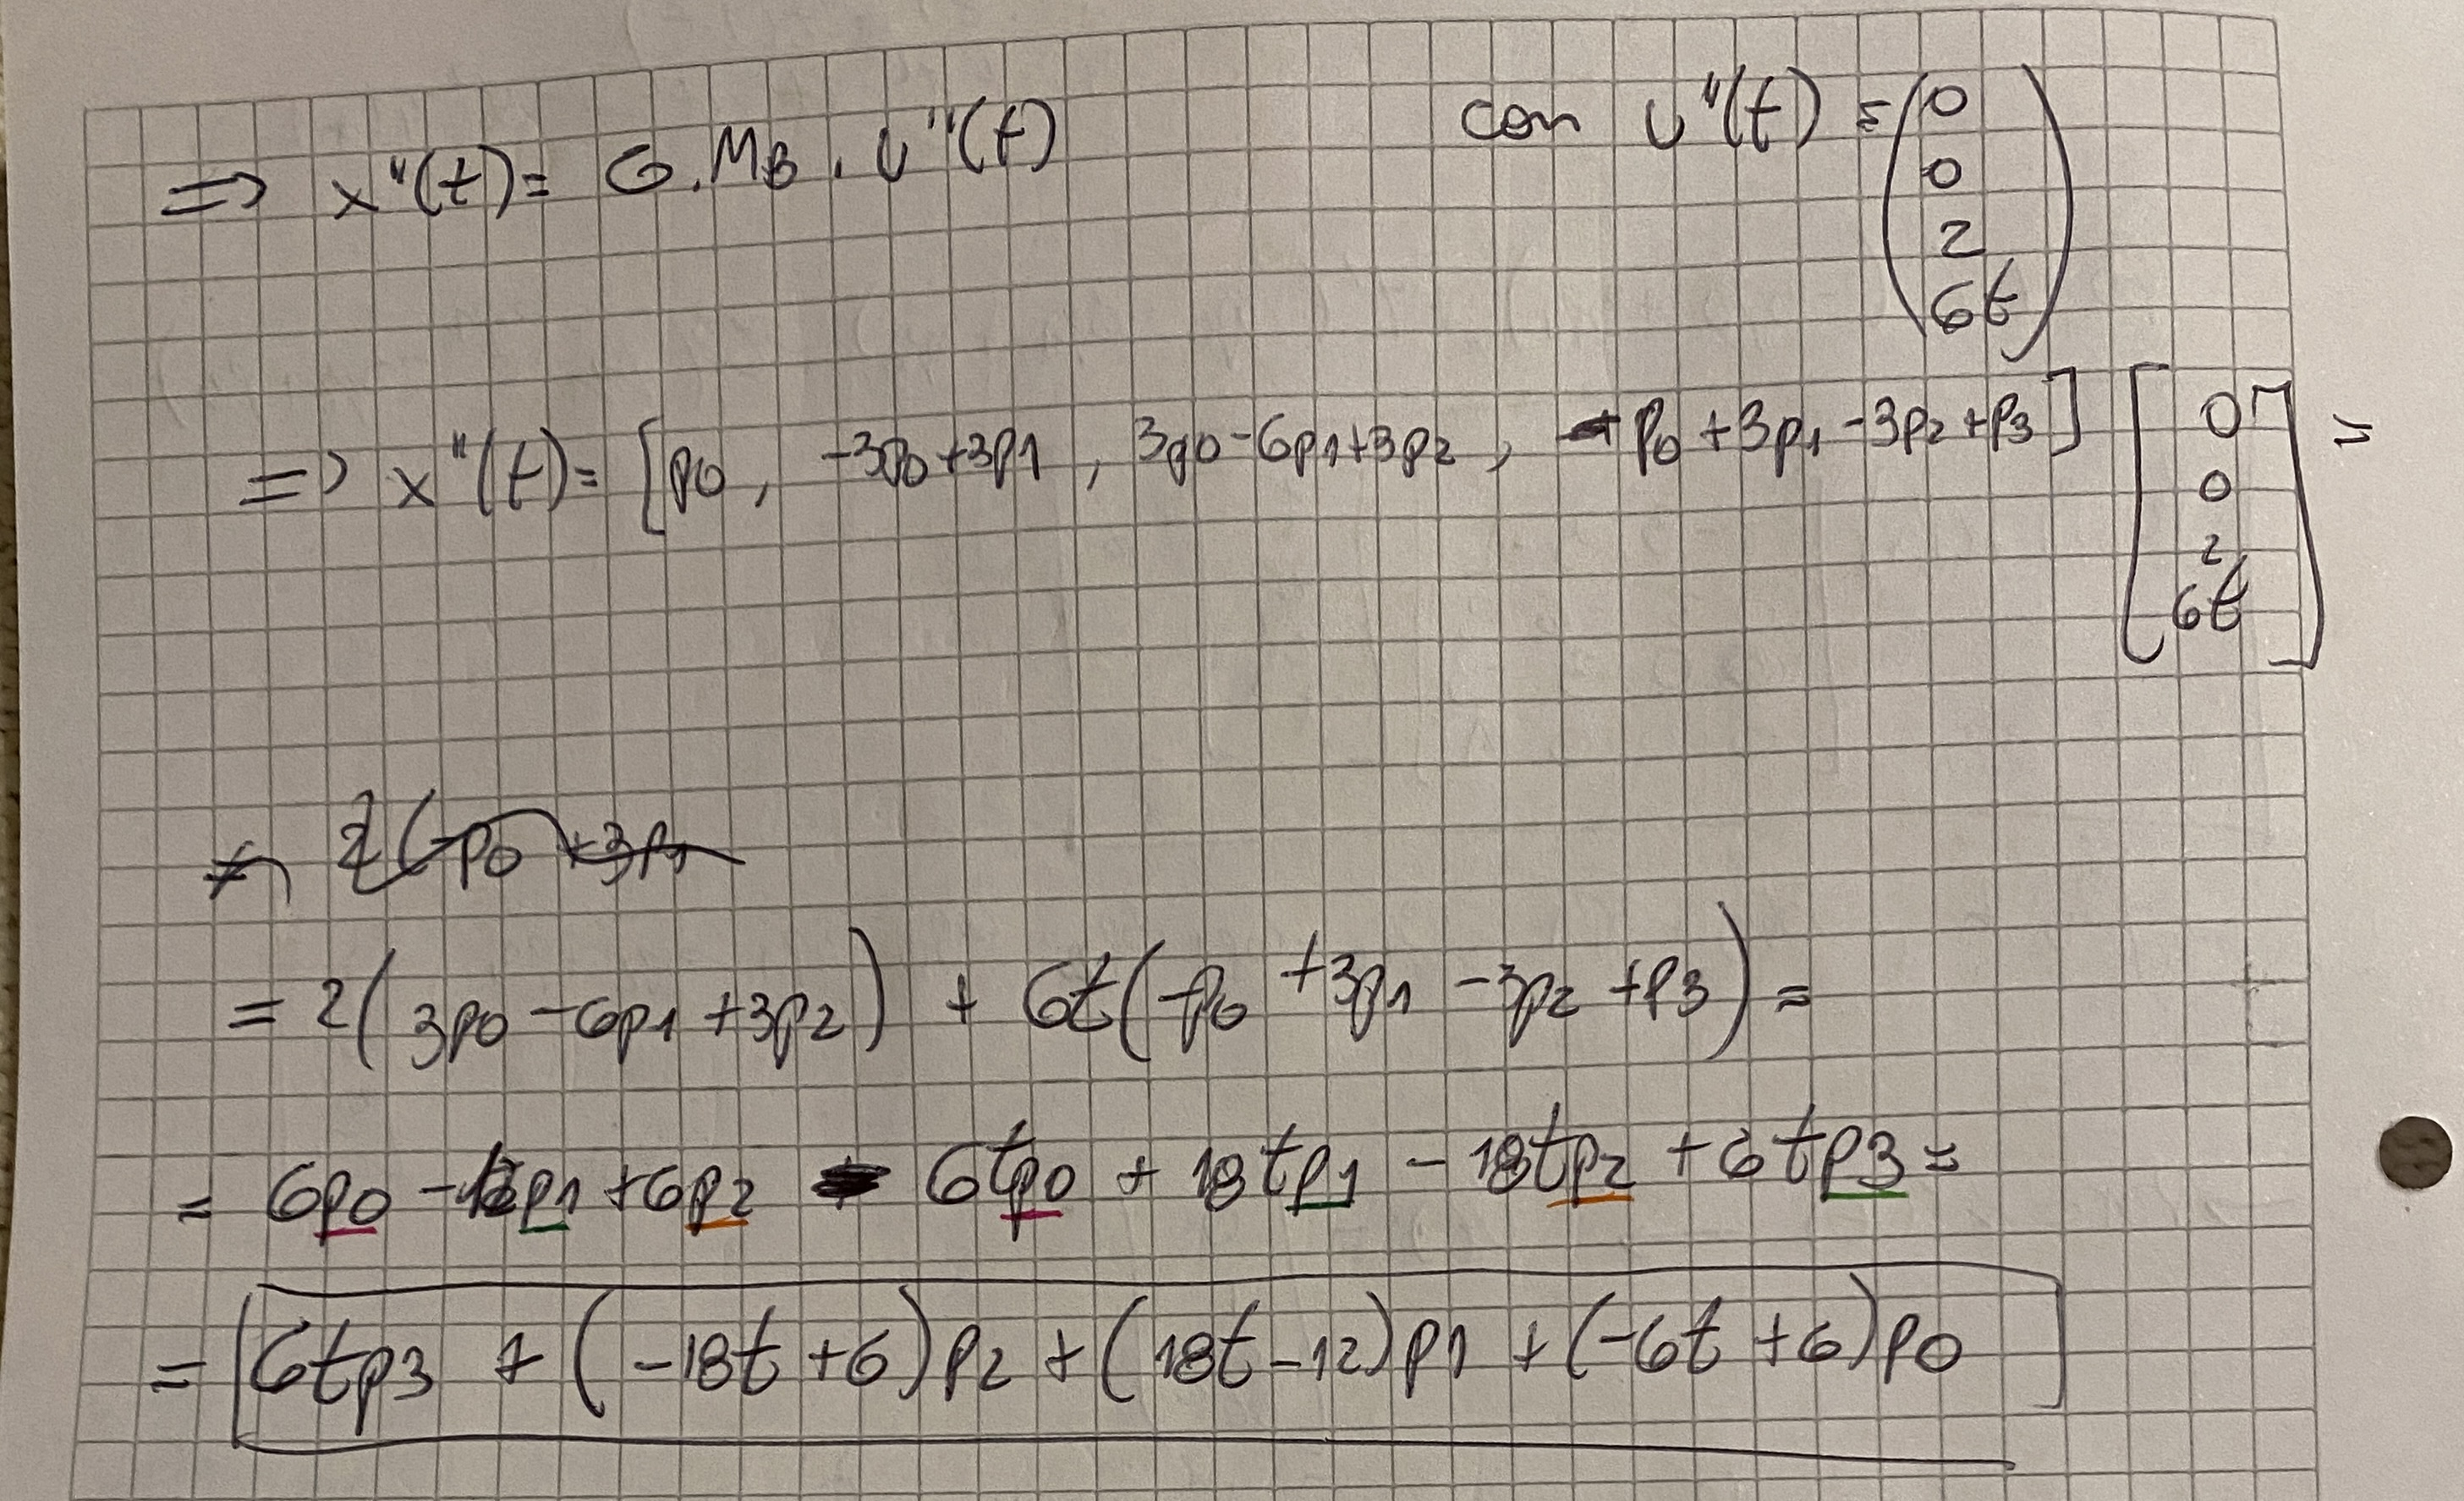
\includegraphics[width=\textwidth]{imagenes/segderiv.jpg}
        \caption{Desarrollo de $x''(t)$}
        \label{fig:grafico2}
    \end{minipage}
    \label{fig:dos_graficos}
\end{figure}

Así, las expresiones desarrolladas para $x'(t)$ y $x''(t)$ son:

\begin{itemize}
    \item $x'(t) = p_0(-3 + 6t - 3t^2) + p_1(3 - 12t + 9t^2) + p_2(6t - 9t^2) + p_3(3t^2)$
    \item $x''(t) = p_0(6 - 6t) + p_1(-12 + 18t) + p_2(6 - 18t) + p_3(6t)$
\end{itemize}

Para determinar cómo se relaciona el vector tangente de la curva de Bézier x(t) con los puntos de control de la curva en t=0 y t=1, evaluamos $x'(t)$ en $t = 1$ y $t = 0$, obteniendo $x'(0) = 3p_1-3p_0$ y $x'(1) = 3p_2-3p_2$. Los vectores tangentes son:
\begin{itemize}
    \item En $t = 0$, $p_0 + (3p_1-3p_0) = 3p_1-2p_0$ (porque el vector pasa por el punto $p_0$).
    \item En $t = 1$, $p_3 +  (3p_3-3p_2) =  4p_3-3p_2$ (porque el vector pasa por el punto $p_3$).
\end{itemize}

A continuación mostramos un ejemplo de una curva de Bézier (la definida por los puntos $p_0 = (1, 6)$, $p_1 = (4, 9)$, $p_2 = (3, 9)$, $p_0 = (1, 0)$) y sus vectores tangentes en $t = 0$ y $t = 1$. El código que genera el gráfico esta en el .ipynb en la sección "Ejercicio 4".

\begin{figure}[H]
    \centering
    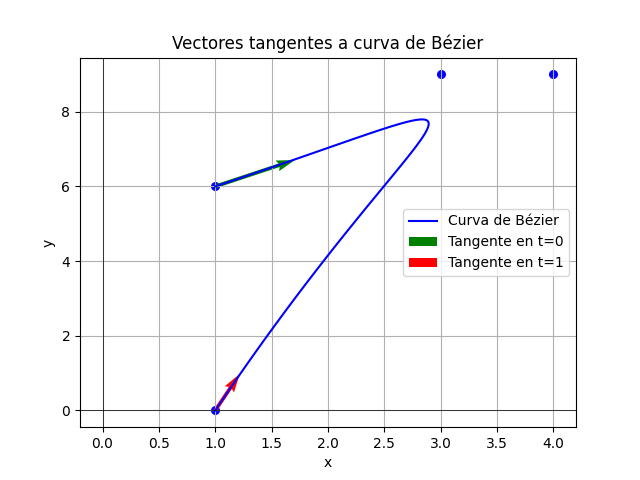
\includegraphics[width=0.6\textwidth]{imagenes/ej4.png}
    \caption{Ejemplo de vectores tangentes a curva de Bézier}
    \label{fig:ejemplo}
\end{figure}

\section*{Ejercicio 5:}
Para que la curva compuesta por $x(t)$ e $y(t)$ sea $C^1$, necesitamos $x'(1) = y'(0)$, para garantizar la existencia y continuidad de la derivada de la curva compuesta en el punto donde se unen $x(t)$ e $y(t)$, que es $p_3 = x(1) = y(0)$. Del ejercicio 4, sabemos que $x'(1) = 3p_3-3p_2$ y que $y'(0) = 3p_4-3p_3$ (haciendo los remplazos necesarios de los puntos de control, es decir $p_3$ como $p_0, p_4$ como $p_1$, etc).

Entonces, debe cumplirse,

$$
\begin{aligned}
x'(1) &= y'(0) \\
3p_3 - 3p_2 &= 3p_4 - 3p_3 \\
2p_3 &= p_4 +p_2
\end{aligned}
$$

Para el segundo ítem, cuando $x'(1) = y'(0) = 0$, se cumple que $x'(1) = 3p_3 - 3p_2 = 0$ por lo que $p_3 = p_2$. Similarmente, $y'(0) = 3p_4 - 3p_3 = 0$ por lo que $p_4 = p_3$. Entonces, cuando $x'(1) = y'(0) = 0$, se cumple $p_2 = p_3 = p_4$.

Para el tercer ítem, si la curva tiene continuidad $C^2$, debe cumplirse que tiene continuidad $C^1$ y que la derivada segunda de la curva compuesta es continua en $p_3$.  

\end{document}


